\documentclass[10pt,a4paper]{article}
\usepackage[utf8]{inputenc}
\usepackage{amsmath}
\usepackage{amsfonts}
\usepackage{amssymb}
\usepackage{caption}
\usepackage{subcaption}
\usepackage{graphicx}
\usepackage[left=2cm,right=2cm,top=2cm,bottom=2cm]{geometry}
\begin{document}
	
	\section*{Subfigure Demo} 
	
	
	\begin{figure}[h]
		\centering
		\begin{subfigure}[b]{0.3\textwidth}
			\centering
			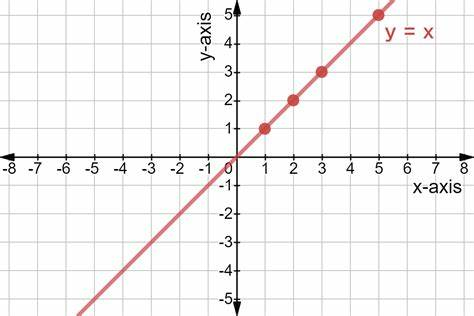
\includegraphics[width=\textwidth]{D:/latex all complete pr/1.jpg} 
			\caption{$y=x$}
			\label{fig:y equals x}
		\end{subfigure}
		\hfill
		\begin{subfigure}[b]{0.3\textwidth}
			\centering
			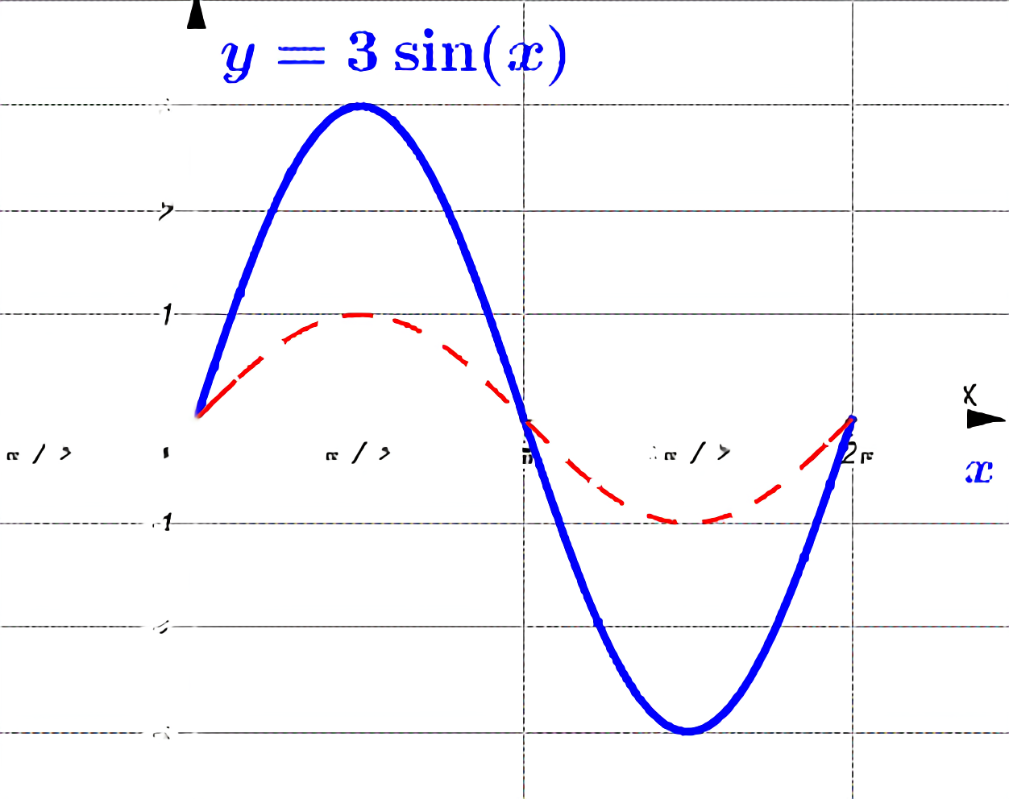
\includegraphics[width=\textwidth]{D:/latex all complete pr/2.png}
			\caption{$y=3\sin x$}
			\label{fig:three sin x}
		\end{subfigure}
		\hfill
		\begin{subfigure}[b]{0.3\textwidth}
			\centering
			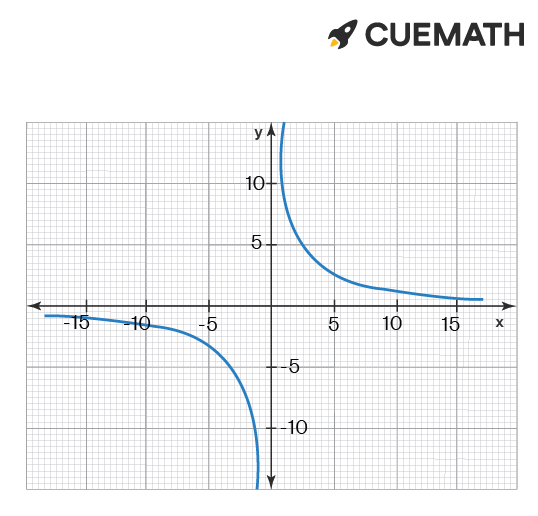
\includegraphics[width=\textwidth]{D:/latex all complete pr/3.png}
			\caption{$y=5/x$}
			\label{fig:five over x}
		\end{subfigure}
		\caption{Three simple graphs arranged side-by-side}
		\label{fig:three graphs}
	\end{figure}
	
\end{document}